%%
% The BIThesis Template for Bachelor Graduation Thesis
%
% 北京理工大学毕业设计(论文)第二章节 —— 使用 XeLaTeX 编译
%
% Copyright 2020-2023 BITNP
%
% This work may be distributed and/or modified under the
% conditions of the LaTeX Project Public License, either version 1.3
% of this license or (at your option) any later version.
% The latest version of this license is in
%   http://www.latex-project.org/lppl.txt
% and version 1.3 or later is part of all distributions of LaTeX
% version 2005/12/01 or later.
%
% This work has the LPPL maintenance status `maintained'.
%
% The Current Maintainer of this work is Feng Kaiyu.
%%

\chapter{基于树状区块链的跨子链转账测试}

\section{树状区块链的跨子链转账}

树状区块链,乃是以区域索引区块链为基础,旨在解决传统区块链单链结构面对大量区块时产生高昂性能代价的痛点。其借助Geohash技术,编码地理位置,并借此对区块链进行划分,形成类似于字典树的树状结构。

然而,这样的结构带来了一个问题:若某个账户的位置发生了较大改变,以至于它离开了目前所在的子链的管辖范围(即账户所在子链表示的Geohash范围不再是账户实际位置的Geohash编码表示的前缀),那么账户在新地理位置上发送的所有交易将失败,因为在逻辑上账户并不由管辖新地理位置所在片区的区块链直接管辖,后者可能根本没有关于该账号的任何记录,或者其上与该账户关联的信息并非切实。

对此,树状区块链的解决方案是:账户需要向一个特殊的管理账号发送一种特殊的交易,该交易及其携带的信息足以令管理账号从账户原先所在的区块链中,将账户的余额信息转移到新区块链上。此后,该账户由新区块链接手管辖,可以正常进行诸如发送交易等的区块链交互操作。由于上述转账过程与同一区块链内两不同账户间的转账不同,乃是横跨两个区块链的、同一账户之间的转账,故称该特殊转账过程为“跨子链转账”。

显然,在尝试解决单链结构的效率问题的同时,树状区块链引入了跨子链转账所需的额外时间开销。跨子链转账操作的效率,将对用户的使用体验有较大的影响。因此,本章将围绕跨子链转账这一主题进行探究。首先,设计并进行数组跨子链转账测试实验;其中,以较小规模的10账号跨子链转账实验测试跨子链转账的正确性;验证正确性后,再开展更大规模的跨子链转账测试,检验跨子链转账操作在不同压力情况下的运行效率波动;最后,给出一个简单的数学模型,探究树状区块链跨子链转账代价与其链上数据查询复杂度降低带来的性能优势基本持平时的临界条件,进而给出适用树状区块链代替传统单链结构区块链的应用场景建议。

\section{测试设计思路}

跨子链转账测试实验将在如图3-1所示的区块链网络中进行。

\begin{figure}[htbp]
    \centering
    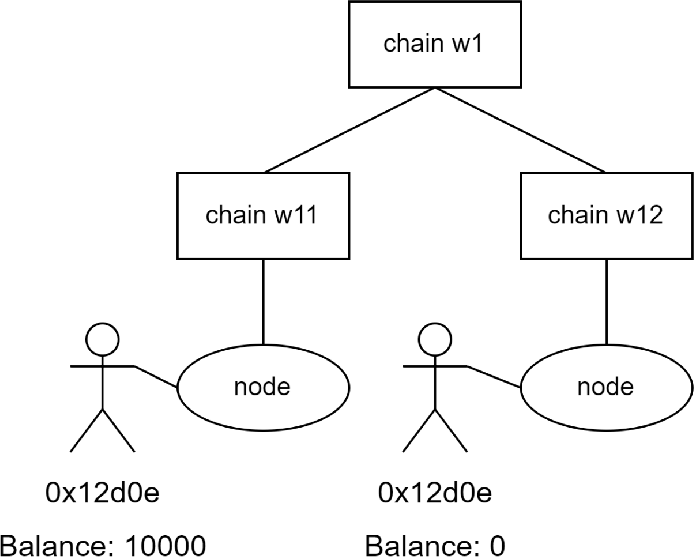
\includegraphics[width=0.5\textwidth]{images/2leaf-structure.png}
    \caption{双子链树状区块链结网络结构}\label{2leaf结构} % label 用来在文中索引
\end{figure}

该区块链网络共由三个链组成,分别以链w1,链w11和链w12指代。链w1为树状区块链中的分支区块链,其管辖的地理位置范围为Geohash编码为w1的所有区域;由链w1负责串联的子链w11、子链w12均为叶子区块链,分别管辖Geohash编码前缀为w11、w12的所有区域,其下分别运行有一个节点,可以同传统区块链节点一样进行挖矿、交易等操作。初始时,两子链中存在相同的数个账号(类似图\ref{2leaf结构}中,位于不同子链下的同公钥账户0x12d0e),但w11中的账号均有$10000$单位的余额,w12中的账号的余额均为0,模拟账号所有者进行了大范围物理位置变动后,尚未转移余额给管辖新地理位置的子链的情况。跨子链转账开始后,待所有链w11中的账号同时发起转账申请后,树状区块链将开始串行地遍历所有子链w11中的账号,并将它们在链w11的余额全部转移至链w12的对应账号之下。待转账完成之后,检查链w12中各账户的余额,即可证明跨子链转账的功能正确性。

在此过程中,监控程序将记录所有账号发起转账申请的时间戳、以及转账完成时的时间戳。通过分析以上数据,即能得到每个账号从串行处理开始至转账完成所花费的总时间,进而在初始待转账账号数量不同时,得出树状区块链在不同工况下的跨子链转账效率。

本测试将从10个账号的小规模跨子链转账测试开始,测试在小压力工况下跨子链转账功能是否运转正常;在此基础上,继续开展20账号,40账号,80账号,120账号,160账号及200账号跨子链转账实验,探究面对不同压力工况时树状区块链的性能表现变化。

\section{环境配置}

跨子链转账测试的测试环境如表3-1所示。

\begin{table}[htbp]
    \linespread{1.5}
    \zihao{5}
    \centering
    \caption{跨子链转账测试环境}\label{跨子链转账测试环境}
    \begin{tabular}{r|l} \toprule
        中央处理器 & Intel Core i5-12500H      \\
        图形处理器 & Intel Iris Xe 80EU        \\
        内存    & 24GB                      \\
        操作系统  & Ubuntu 22.04.2 LTS        \\
        虚拟机   & VMWare Workstation Pro 17 \\
        \bottomrule
    \end{tabular}
\end{table}

另外,还需安装\verb|make|程序包,并下载树状区块链的源代码\footnote{\url{https://github.com/xyongcn/BlockChain2017/tree/master/src/go-ethereum1.9.12-modify/go-ethereum}}。

\section{测试步骤}

\subsection{编译并配置树状区块链}

下载源代码后,在源代码目录启动终端,输入\verb|make geth|,等待编译完成,即能在\verb|build/bin|目录中发现geth二进制可执行文件。将其重命名为geth-tree,并复制到\verb|/usr/local/bin|目录中。

\subsection{进行测试}

代码仓库\footnote{\url{https://gitee.com/endericedragon/transfer-2leaf}}给出了构建图3-1所示的区块链网络的数据文件和脚本,并附有一份实验手册。本节将简要介绍测试步骤。


\begin{enumerate}
    \item 确认w1、w11和w12的数据目录中不存在\verb|gethdata/geth|子目录。若存在,则需要将其删除;
    \item 在代码仓库根目录中启动终端,运行\verb|sh w1_init.sh|指令,启动分支区块链w1,并留意形如INFO [04-10|20:36:48.833] Started P2P networking self="enode://......"的输出,记录该双引号包裹的字符串;
    \item 在链w11和链w12的预加载脚本中,替换\verb|admin.addPeer()|方法的参数为上一步中记录的字符串
    \item 另启动两个终端,分别执行启动链w11和链w12的脚本,若观察到形如\begin{verbatim}
INFO [04-10|20:54:02.335] Block synchronisation started
---k:aaaaaaaaaaaaw1,v.RegionId:w1,v.Number:1---
---parent.Number:0, branchb.RegionId:w1,ptd:131072---
!!commitBranchBlock[aaaaaaaaaaaaw1][1]--[td:262144]success!!
    \end{verbatim}
          字样,即为子区块链和父区块链同步成功,可以进行下一步骤的实验;
    \item 另启动一个终端,运行\verb|branchnode-remastered.js|脚本。该脚本将监视父区块链w1的日志内容,并根据之运行相应代码,完成转账等操作;
    \item 在链w11和链w12中启动挖矿后,启动一个终端,执行\verb|node transfer_test_step1.js|指令。该指令将从链w11的矿工账号,分别为链上的其他账号转账10000单位的资产作为初始资金,在接下来的步骤中,这些资产将被转移到链w12中的同名账号上;
    \item 确认初始资金全部到位后,执行\verb|node transfer_test_step2.js|,终端中将出现与挖矿提示\verb|line:--handler-TX_request--|不同的输出,等待,直至终端仅输出挖矿提示;
    \item 执行\verb|node query_transfer_time_w11_w12.js|,脚本将访问链w11和链w12上的所有区块,统计其中包含的交易及其详细信息,生成测试结果报告。
\end{enumerate}

\section{测试结果分析}

使用\verb|eth.getBalance(accountAddress)|函数,可以在Geth的JavaScript控制台中年轻松地查看给定账号的余额,进而检查转账是否成功。本章所有测试均已确认在跨子链转账结束后,原链w11中各账户的余额均为0,而链w12中的对应账户余额为10000单位,从而证明了跨子链转账功能的正确性。

由于测试设计为将账户余额从链w11转账到链w12中,故在生成的测试报告中,仅需关注\verb|tx_request_w12.txt|和\verb|tx_result_w11.txt|文件即可。前者记录了发起转账申请的时间戳,由于所有账号乃是同时发起转账申请,故所有条目的时间戳均相同;后者记录了各账户在链w12真正收到资产的时间戳。根据后者(即\verb|tx_result_w11.txt|文件),可以轻松重建树状区块链串行处理所有账户的顺序,以及处理各个账户分别花费的时间。

\subsection{小规模跨子链转账测试结果分析}

本文以10账号参与的跨子链转账测试结果作为小规模跨子链转账测试的测试结果。根据测试报告内容,所有10个账号均在时间戳1683465655发起转账申请,但在链w12上收到资产的时间戳不同,数据如下:

\begin{table}[htbp]
    \linespread{1.5}
    \zihao{5}
    \centering
    \caption{10账号测试结果}\label{10账号测试结果}
    \begin{tabular}{*{5}{>{\centering\arraybackslash}p{6cm}}} \toprule
        账号公钥地址                                     & 收到资产的时间戳   \\\hline
        0x4461e120a1bcbdc9e08730f59c7e169bac5de38f & 1683465667 \\
        0x59cadf05182c56784b60960159c0fb4d16860d10 & 1683465680 \\
        0x8ed2d00a4ee496e51fab00ddc7561f85186e2a9c & 1683465688 \\
        0x95fcbbba05858b53b829361a052450179d7a62ca & 1683465694 \\
        0xcada164cb319316a133741dbaa1b40fcc8caec52 & 1683465703 \\
        0x1daf02e444bec7fc7fdbbac7704c57d001b19648 & 1683465711 \\
        0x023bc9309e89678b5de3ea084a5a91cc0679dd39 & 1683465720 \\
        0x4d326e5422c48ca1db8695bb59c9a58005a3fb44 & 1683465724 \\
        0x12d0e4381ef94a70a49252e35b9a65fadd3872b9 & 1683465735 \\
        0x0b424be2eb61a4fa045161198754613a93845857 & 1683465743 \\
        0xf41384cb20cd007daea6b0d7eefa3942ac44a3d1 & 1683465750 \\
        \bottomrule
    \end{tabular}
\end{table}

结合发起转账请求之时间戳,可以计算得到树状区块链为每个账户办理转账所花费的时间。笔者使用形如附录C的Python代码进行可视化,如图3-2所示:

\begin{figure}[htbp]
    \centering
    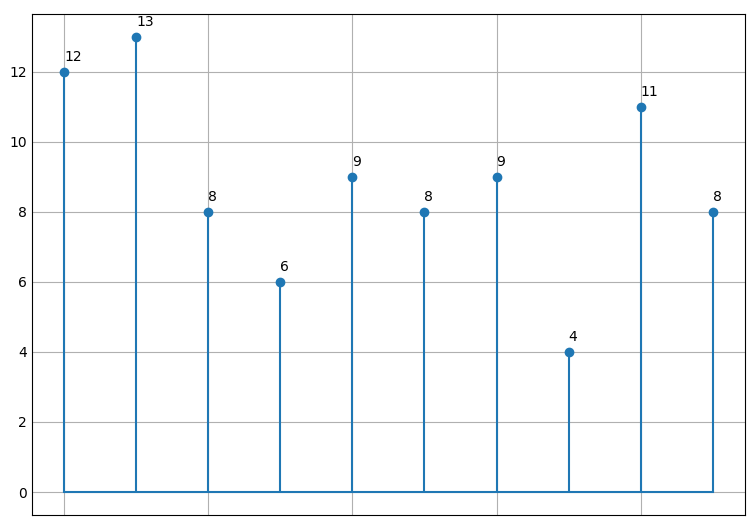
\includegraphics[width=\textwidth]{images/10accounts.png}
    \caption{10账号跨子链转账测试的可视化}\label{10账号跨子链转账测试的可视化} % label 用来在文中索引
\end{figure}

根据图3-2计算,得到如下测试数据:

\begin{table}[htbp]
    \linespread{1.5}
    \zihao{5}
    \centering
    \caption{10账号测试数据}\label{10账号测试数据}
    \begin{tabular}{*{5}{>{\centering\arraybackslash}p{6cm}}} \toprule
        总耗时(秒)          & 95     \\
        最快转账处理速度(秒)     & 4      \\
        最慢转账处理速度(秒)     & 13     \\
        平均转账处理速度(秒)     & 8.8000 \\
        转账处理速度方差(秒$^2$) & 6.5600 \\
        \bottomrule
    \end{tabular}
\end{table}

观察图3-2不难发现,虽然10个账号的转账申请确实是同时发起的,但由于以太坊仅能串行处理的特性,导致从第一份转账请求发起,到最后一次转账交易完成并写入区块为止的总耗时较为夸张。同时,参与测试的10个账号之转账处理时间方差较大,最快转账处理速度较最慢处理速度的差距足有9秒。

\subsection{大规模跨子链转账测试结果分析}

随着请求转账的账号数量增加,其转账处理效率是否会随之变化?本文继续以类似的方法,开展了20账号、40账号、80账号、120账号、160账号、200账号的跨子链转账测试。由于篇幅限制,本节将不展示可视化图示,仅展示经过计算得出的统计数据。

\begin{table}[htbp]
    \linespread{1.5}
    \zihao{5}
    \centering
    \caption{测试数据汇总}\label{测试数据汇总}
    \begin{tabular}{r|c|c|c|c|c|c} \toprule
                        & 20账号   & 40账号    & 80账号    & 120账号  & 160账号   & 200账号   \\\hline
        总耗时(秒)          & 163    & 319     & 654     & 978    & 1363    & 1621    \\
        最快转账处理速度(秒)     & 4      & 2       & 1       & 2      & 1       & 1       \\
        最慢转账处理速度(秒)     & 16     & 17      & 21      & 17     & 27      & 21      \\
        平均转账处理速度(秒)     & 9.0556 & 8.6216  & 8.9589  & 8.5789 & 8.5188 & 8.7622  \\
        转账处理速度方差(秒$^2$) & 8.0525 & 11.0460 & 19.0805 & 8.3666 & 25.9446 & 12.8407 \\
        \bottomrule
    \end{tabular}
\end{table}

观察表3-4的数据,可以提出以下猜想:
\begin{itemize}
    \item 转账过程耗时和参与转账的账号存在线性关系;
    \item 虽然转账处理速度方差较大,但平均处理速度较为稳定,大约在8.5秒到9.1秒之间。
\end{itemize}

其中,第二个猜想可以从表3-4中较直观地得到,故本文将重点讨论第一个猜想的验证。

\subsubsection{验证转账耗时和账号数量的线性关系}

本文使用最小二乘法进行线性拟合计算。记账号数量为$x$,假设$time_\theta(x)$为$x$个账号跨子链转账需要花费的时间,那么后者可以写作:

$$
    time_\theta(x) =
    \begin{bmatrix}
        1 & x \\
    \end{bmatrix}
    \cdot
    \begin{bmatrix}
        \theta_0 \\
        \theta_1
    \end{bmatrix}
$$

根据最小二乘法:

$$
    \vec{\theta} = (\vec{X}^T \vec{X})^{-1}\vec{X}^T \cdot \vec{Y}
$$

其中,$\vec{X}$,$\vec{Y}$是分别为样本的输入向量和输出向量。根据以上算法,可得本例中的各个向量为:

$$
    \vec{X} = \begin{bmatrix}
        1 & 20 \\ 1 & 40 \\ 1 & 80 \\ 1 & 120 \\ 1 & 160 \\ 1 & 200
    \end{bmatrix} \\
    \vec{Y} = \begin{bmatrix}
        163 \\ 319 \\ 654 \\ 978 \\ 1363 \\ 1621
    \end{bmatrix}
$$

带入最小二乘法公式进行计算,可得:

$$
    \theta = \begin{bmatrix}
        -4.68767123 \\
        8.26794521
    \end{bmatrix} \\
$$
$$
    R^2 = 1 - \frac{\sum_i (y_i - \overline{y})^2}{\sum_i (y_i - times_{theta}(x_i))^2} = 0.9982362552443657
$$

其中,$x_i$,$y_i$代表$\vec{Y}$的各个水平分量,$\overline{y}$代表$\vec{Y}$的算术平均值。

拟合度$R^2$非常接近1,这正证明了自变量——账号数量$x$和因变量——跨子链转账耗时$time_theta$确实可以在统计学上认为存在线性关系$time_{\theta}(x) = -4.68767123 + 8.26794521 \cdot x$,进而验证了以太坊顺序串行处理收到的所有交易的特点。

\section{基于测试结果进行数学建模}

传统区块链单链结构的查询效率低,但胜在无需额外操作维护正确的账户状态;而树状结构的查询效率高,但引入了跨子链转账的额外开销。根据使用场景的不同,用户需要在上述两种区块链实现中恰当进行选择,方能在特定的应用场合获得更好的使用体验。本节将基于已收集的测试数据,建立简单的数学模型,探讨在不同场景下使用树状区块链和传统区块链的理论性能差异,为用户在两种区块链实现之间的选择提供建议。

\subsection{静态查询复杂度分析}

静态查询复杂度分析,约束所有账号的地理位置不发生变化,因此不会考虑跨子链查询的情况。本小节将基于以上约束,讨论单链结构区块链和树状区块链查询信息的复杂度情况。

在单链结构区块链下,所有链上信息均存储在同一条链中。若进行一次查询,最坏情况下需要遍历整条链才能获得结果。记总区块数为$n$,则该过程的平均时间复杂度为$O(n)$。

在树状区块链下,情况较为复杂,为简单起见,本节讨论一条父链,$x$条子链组成的双层树状区块链,并假设所有区块均匀地分布在子链中。仍记总区块数为$n$,那么每条子链中包含$\frac{n}{x}$个区块。此时若进行一次查询,最坏情况下仅需遍历一条子链即可,平均时间复杂度为$O(\frac{n}{x})$。

注意到当分母$x$越大,查询的时间复杂度越低。这是因为,在区块均匀分布的前提下,数状结构的深度随分支的增加而减少。结合树状区块链分支的实际意义,可以得到以下结论:

\begin{itemize}
    \item 当链上交易发生的地理位置跨度较大,且在各地理位置范围分布较均匀时,适合使用树状区块链而非单链结构区块链;
    \item 当链上交易发生的地理位置非常集中时,树状区块链的表现和单链结构区块链接近,故无需使用树状区块链。
\end{itemize}

\subsection{动态查询复杂度分析}

动态查询复杂度分析,假设节点在树状区块链的各子链间周期性移动,从而将跨子链这一开销纳入考量。本小节中,将针对节点中的一个账号进行分析。该账号行为描述如下:处于某一条子链中时,进行数笔交易,这些交易分别记录在不同的区块中。随后,账号立即转移前往下一个子链,此时若进行查询操作,必须先进行跨子链转账,将该账户之余额转移到新子链上,然后再进行查询。

在单链结构区块链下,情况与静态查询情况类似,进行一次查询,最坏情况下仅需遍历一条子链即可,平均时间复杂度为$O(n)$。

在树状区块链下,情况更为复杂。记$lcm(c, q)$为账号跨子链的间隔之间产生的区块数量$q$和查询间隔之间产生的区块数$c$的最小公倍数,那么在产生$lcm(c, q)$个区块的过程中,将发生$\frac{lcm(c, q)}{c}$次查询,且账号将进行$\frac{lcm(c, q)}{q}$次跨子链移动。那么$\frac{lcm(c, q)}{c}$次查询的总时间复杂度为$O(q \times \frac{lcm(c, q)}{c}) + \frac{lcm(c, q)}{q} \times T_{cross}$,其中$T_{cross}$为单个账户跨子链转账的时间开销。那么,平均到每一次查询的时间开销即为$(O(q \times \frac{lcm(c, q)}{c}) + \frac{lcm(c, q)}{q} \times T_{cross}) \times \frac{c}{lcm(c, q)} = O(q) + \frac{c}{q} \times T_{cross}$。

令$lcm(c, q) = n$,比较两区块链实现在生成相同区块数量下的复杂度表现,列不等式:

$$
    O(lcm(c, q)) \geq O(q) + \frac{c}{q} \times T_{cross}
$$

由于在遍历长为$length$的区块链链条时,可以认为找到目标区块的期望复杂度为$\frac{length}{2}$;同时,经过实测,$T_{cross}$的值可以取表3-4中跨子链转账测试的平均处理速度的平均值(经过计算,大约8.7493秒),故可以改写上述不等式为:

$$
    \frac{lcm(c, q)}{2} \geq \frac{q}{2} + \frac{c}{q} \times 8.7493
$$

当满足上述不等式时,树状区块链更有可能提供相较传统区块链更优越的性能。

观察树状区块链的动态查询复杂度表达式可知,当查询非常频繁,即$c$的值变小时,复杂度将相应降低。

注意到,$q$的增大在$O(q)$中,对时间复杂度起到增加作用,却在$\frac{c}{q} \times acc \times T_{cross}$中起到减少时间复杂度的作用。这是因为,增大$q$相当于容许子链拥有更长的长度,账号所有者停留在同一子链中的时间延长,也就相应减少了跨子链转账操作的次数。因此,即便是在树状区块链中,用户也需要合理设计子链的管辖范围,将节点跨子链的频率控制在合理的区间内。

综上所述,在下列场景中,选择树状区块链将比选择单链结构区块链更优:

\begin{itemize}
    \item 账号的地理位置变化频率适中;
    \item 数据查询请求量较大。
\end{itemize}

\section{本章小结}

本章介绍了树状区块链为保证子链间数据一致性而生的新概念——跨子链转账操作,介绍了该操作引入的额外时间复杂度。随后,设计并进行了一系列测试,按照压力自小到大的顺序逐步验证了跨子链转账操作的结果正确性、具体测量了该操作带来的额外时间开销,将其可视化并统计整理,进行统计学分析。在分析时,发现并合理利用一些最优化方法验证了参与转账的账户数量与转账耗时的线性关系,证明跨子链转账这一操作为串行处理。最后,分别在静态和动态的场景下建立简单的数学模型,从理论与实际测量数据结合的角度比较了传统单链结构区块链和树状区块链的性能表现,并就在何场景下使用何者给出了一些建议。
